\svnidlong
{$HeadURL: $}
{$LastChangedDate: $}
{$LastChangedRevision: $}
{$LastChangedBy: $}
\svnid{$Id: $}   

All models detailed in this Section are applicable to signatures where 
a photon, a W boson, a Z boson or a Higgs boson
is radiated from the initial state partons instead of a gluon. 
The experimental signature is identified as \textit{V+\MET} and it
has been sought by ATLAS and CMS in Refs.~\cite{Khachatryan:2014rwa,Aad:2014tda,Khachatryan:2014tva,ATLAS:2014wra,Aad:2013oja,Aad:2014vka}. 
This signature is also produced by the models described in 
Section~\ref{subsec:EWSpecificModels}. 

Monojet searches are generally more sensitive
with respect to final states including bosons, due to the much
larger rates of signal events featuring quark or gluon radiation with
respect to radiation of bosons~\cite{Zhou:2013fla},
in combination with the low branching ratios if leptons from
boson decays are required in the final state.
The rates for the Higgs boson radiation is too low for these models
to be considered a viable benchmark~\cite{Carpenter:2013xra}.
However, the presence of photons,
leptons from W and Z decays,
and W or Z bosons decaying hadronically
allow backgrounds to be rejected more effectively,
making Z/gamma/W+\MET searches
still worth comparing with searches in the jet+\MET final state.

In the case of a \spinone mediator,
an example Feynman diagram for these processes can be constructed by taking
Fig.~\ref{fig:OP} and replacing the gluon with $\gamma,W$ or $Z$.

%CD: Peskin killed all of this
%When the initial state radiation is a $W^\pm$ boson, Run~1 searches have considered three benchmark cases adapted from the vector interaction in Ref. ~\cite{Bai:2012xg}, distinguished by $\xi$, the strength of the $d$ quark coupling relative the $u$ quark coupling:
%\begin{itemize}
% \item[$\xi=0$:] Mediator couples to up-type or down-type quarks, but not both;
% \item[$\xi=1$:] Mediator couples to up-type and down-type quarks with same strength;
% \item[$\xi=-1$:] Mediator couples to up-type and down-type quarks with same strength, but opposite sign.
%\end{itemize}
%
%Contemplation of $\xi=-1$ heightened interest in searches for \spinone mediators with $W^\pm$ bosons in the final state. This choice enhances the cross-section significantly above the other choices and hardens the distribution of missing transverse energy used in the searches. The sensitivity of the $W+\MET$ search then surpasses that of the jet$+$\MET search. However, the situation $\xi=-1$ does not appear in an $\mathrm{SU}(2)$-gauge-invariant simplified model.\sidenote{It is well-known that the diagrams in which the $W$ couples to $u$ and $\bar{d}$ have opposite sign. This is what gives rise to the ``helicity zero'' in $u \bar{d} \rightarrow W g$. The relative sign is set by $\mathrm{SU}(2)$ and the statement that the mediator is an $\mathrm{SU}(2)$ singlet. We can increase the cross section by changing the sign, but to do so we have to give the mediator some $\mathrm{SU}(2)$ quantum number, making it, and the associated $\chi$, visible.} The simplified model with a vector mediator exchanged in the \schannel model is still viable when $\xi=1$\sidenote{The $W^\pm$ couples to the initial state quarks as $V$-$A$. If the mediator couples to quarks as $V$+$A$ then one expects the process to vanish completely in the massless quark limit.}. Ref.~\cite{Bell:2015sza} discusses the viability of departures $\xi < 1$ from both gauge-invariance and experimental points of view. An example of a model that arranges different effective DM couplings to $u_L$ and $d_L$ is detailed in Appendix~\ref{app:EWSpecificModels_Appendix}.

When the initial state radiation is a W boson, Run-1 searches have considered three benchmark cases, varying the relative coupling of the $W$ to $u$ and ${d}$ quarks.
The simplified model with a vector mediator mediator exchanged in the s-channel includes only the simplest of these cases, in which the $W$ coupling to $u$ and ${d}$ quarks is identical, as required naively by $\mathrm{SU}(2)$ gauge invariance.  With some more complex model building, other cases are possible.  The case in which the $u$ and ${d}$ couplings have opposite sign is particularly interesting, since this enhances the $W+\MET$ signal over the jet$+$\MET signal~\cite{Bell:2015sza, Bai:2012xg}. Models of this type are discussed in Appendix~\ref{app:monoWExtramodel}.

%The scan in the parameters that characterize this simplified model for EW boson + \MET
%searches follow what is
%already detailed in Section~\ref{subsec:MonojetLikeModels}.


% CD: I tend to like this list so I'll leave it here in hope of recycling it
% \begin{itemize}
%  \item the mass of the DM particle ($m_{DM}$);
%  \item the mediator mass ($m_{Med}$);
%  \item the mediator width ($\Gamma_{Med}$);
%  \item the couplings between the DM and the mediator (\gdm),
%  and between the mediator and the initial state quarks ($g_{SM}$);
%  \item the chirality of the couplings between DM and mediator,
%  and between mediator and initial state quarks (vector-vector, axial-vector, axial-axial, vector-axial).
% \end{itemize}

The results shown in this Section
have been obtained using a LO UFO model in \madgraph 2.2.3 interfaced to \pythiaEight
for the parton shower, as detailed in Section\cite{sec:EW_implementation}
None of these models requires merging samples with different parton multiplicities  
since the visible signal comes from the production of a heavy SM boson whose transverse momentum distribution is sufficiently 
well described at LO+PS level.  As a result, no special runtime configuration is needed for \pythiaEight. 

In these $V$+\MET models, as in the case of the jet+\MET models, \pT of the boson or the \MET does not depend 
strongly on the width of the mediator. An example of the particle-level analysis acceptance using the
generator-level cuts from Ref.~\cite{Aad:2014tda}
for the photon+\MET analysis, but raising the photon $p_T$ cut
to 150~\gev, is shown in Figure~\ref{fig:DMV_EW_gamma_acceptance},
comparing a width that is set to $\Gamma=M_{med}/3$ to the
minimal width (the ratio between the two widths
ranges from 1.05 to 1.5 with increasing mediator masses).

%% Redone as a table.
% mmed : minW
% 10  : 3.5
% 50 : 21.3
% 100 : 42.4
% 300 : 127.3
% 600 : 300.1
% 1000 : 503
% 3000 : 1512
% 6000 : 3024
\begin{table}[!h]
\begin{tabular}{| l |r r r r|}\hline
\multicolumn{5}{|c|}{Acceptance ratio for $\Gamma=\Gamma_{\rm min}$ vs
$\Gamma=\mMed/3$} \\ \hline 
\multicolumn{1}{|c|}{ } & \multicolumn{4}{c|}{\mdm/GeV}\\
\hline 
{\mMed/GeV}      & 10     & 50    & 200   & 400  \\ \hline
50   & 0.96   & 0.99  &       & 0.95 \\  
100  & 0.97   &       &       &      \\
300  & 1.00   & 1.02  &       &      \\
600  &        &       & 0.96  &      \\
1000 & 1.01   & 1.02  & 1.03  &      \\
3000 & 1.02   & 1.03  &       & 1.01 \\
\hline
\end{tabular}
    \caption{Analysis acceptance ratios for the photon+\MET analysis when varying the mediator width, in the
    case of a vector mediator exchanged in the \schannel}%This plot will come from Marie-Helene
    \label{fig:DMV_EW_gamma_acceptance}
\end{table}

%% \begin{figure}
%%     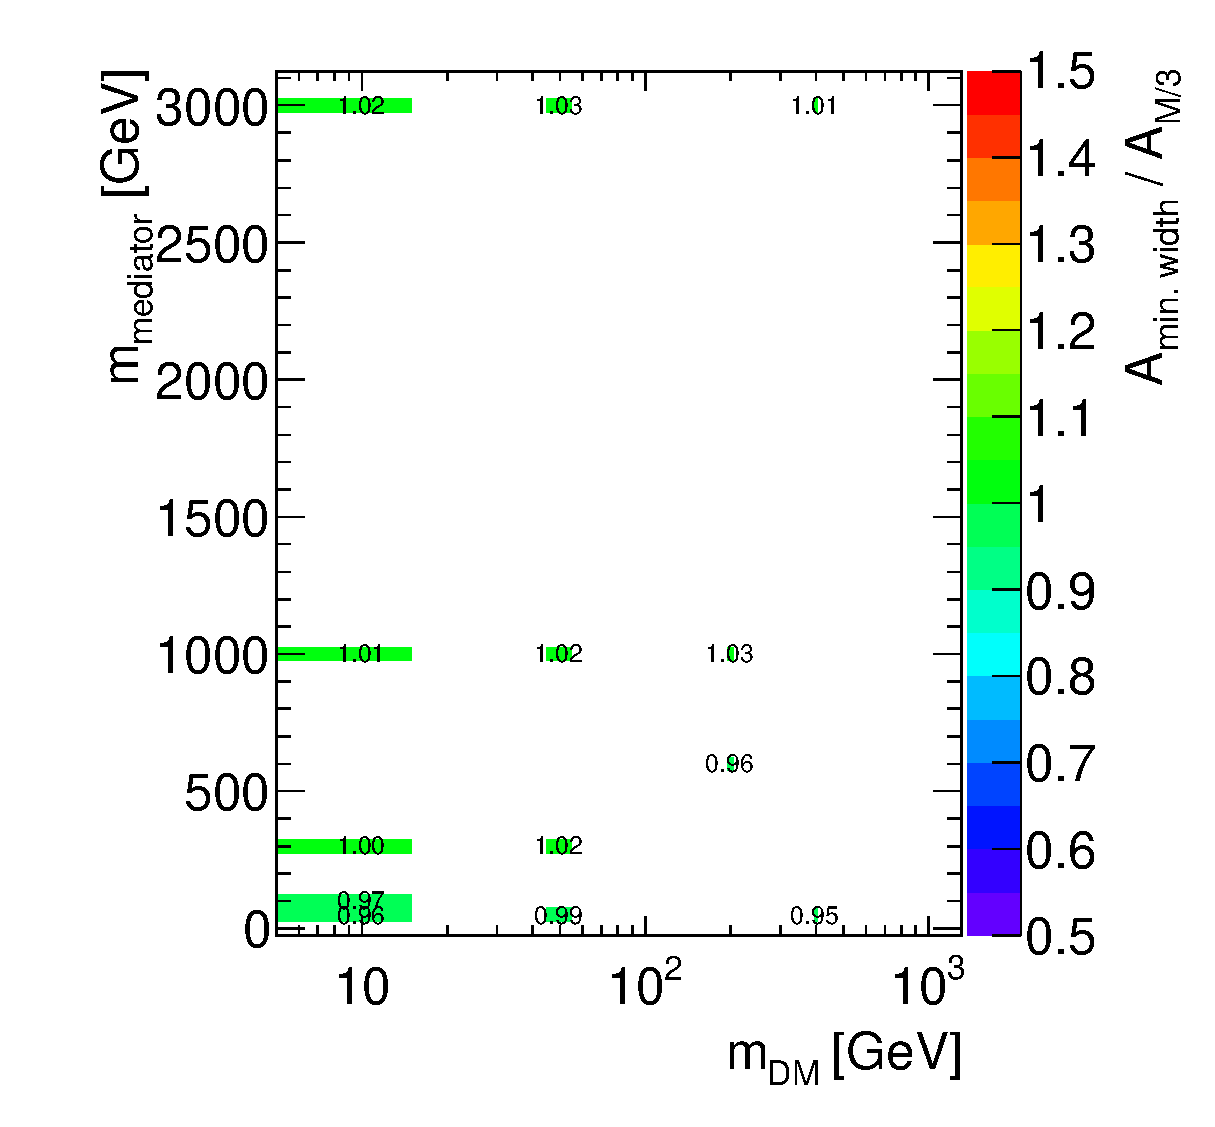
\includegraphics[width=0.7\textwidth]{figures/EW/acceptance_minwidth_vs_mo3_gamma}
%%     \caption{Analysis acceptance for the photon+\MET analysis when varying the mediator width, in the
%%     case of a vector mediator exchanged in the \schannel}%This plot will come from Marie-Helene
%%     \label{fig:DMV_EW_gamma_acceptance}
%% \end{figure}

Examples of relevant kinematic distributions for selected benchmark points are
shown in Fig.~\ref{fig:DMV_EW_kinematics_SVMed}. 

\begin{figure*}[h!]
\centering  
\subfloat[Missing transverse momentum distribution for the photon+\MET final state, for 
different mediator mass choices, for \mdm=10~\gev.\label{fig:DMV_EW_gamma_MET_SVMed}]{%
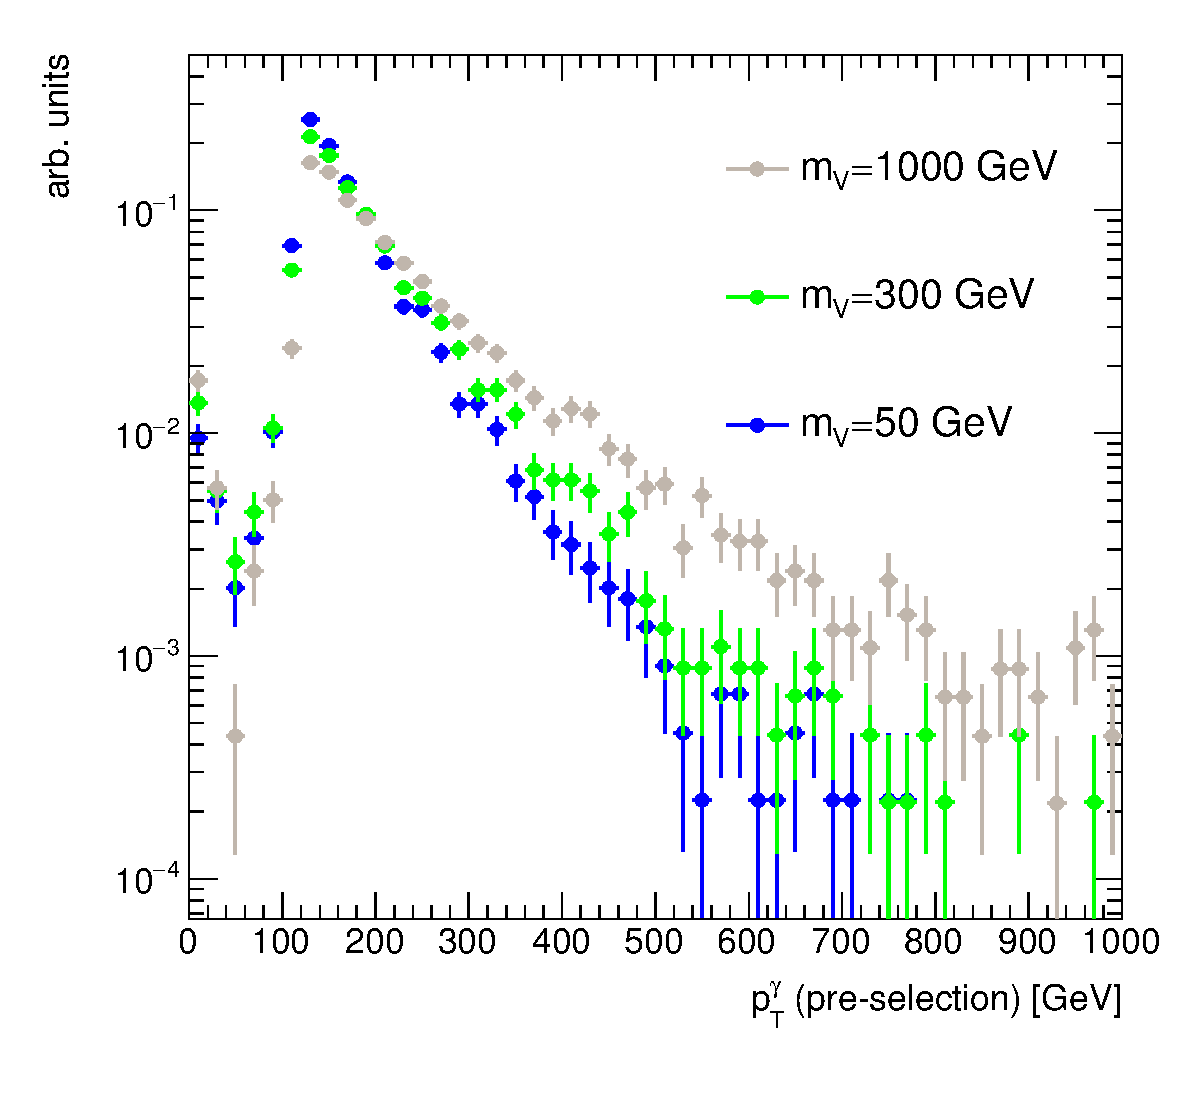
\includegraphics[width=0.49\textwidth]{figures/EW/ptGamma_filter120GeV_dmV_dm10GeV}
}
\hfill
\subfloat[Leading photon transverse momentum distribution for the photon+\MET final state, 
for different DM mass choices, with \mMed=1~\tev.\label{fig:DMV_EW_gamma_pT_SVMed}]{%
		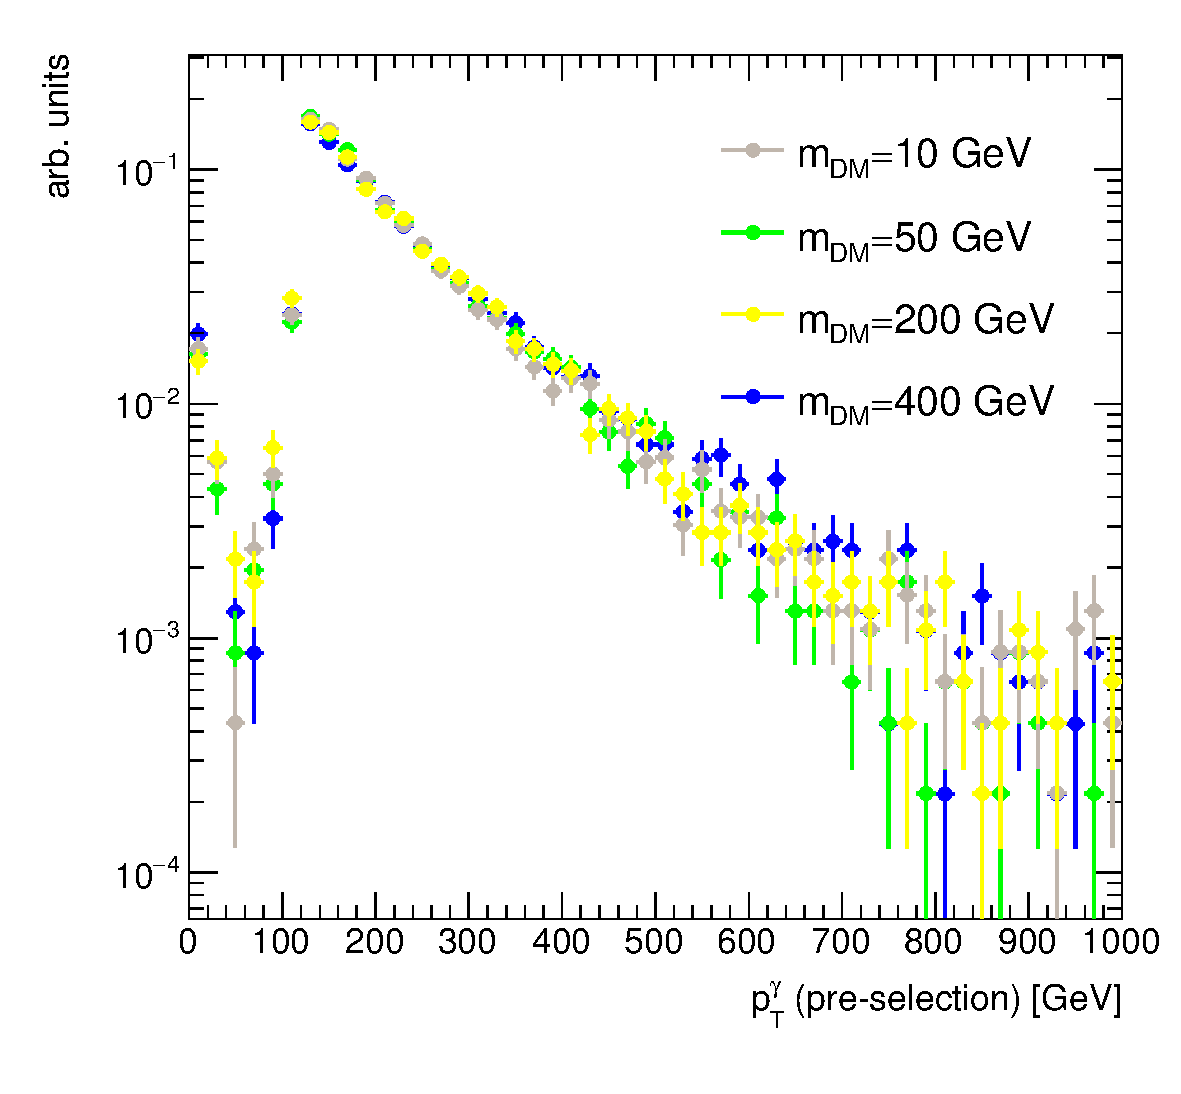
\includegraphics[width=0.49\textwidth]{figures/EW/ptGamma_filter120GeV_dmV_mV1000GeV}
}
\hfill
\subfloat[Missing transverse momentum distribution for the leptonic Z+\MET final state, 
for different mediator mass choices, for \mdm=15~\gev\label{fig:DMV_EW_Z_MET_SVMed}]{%
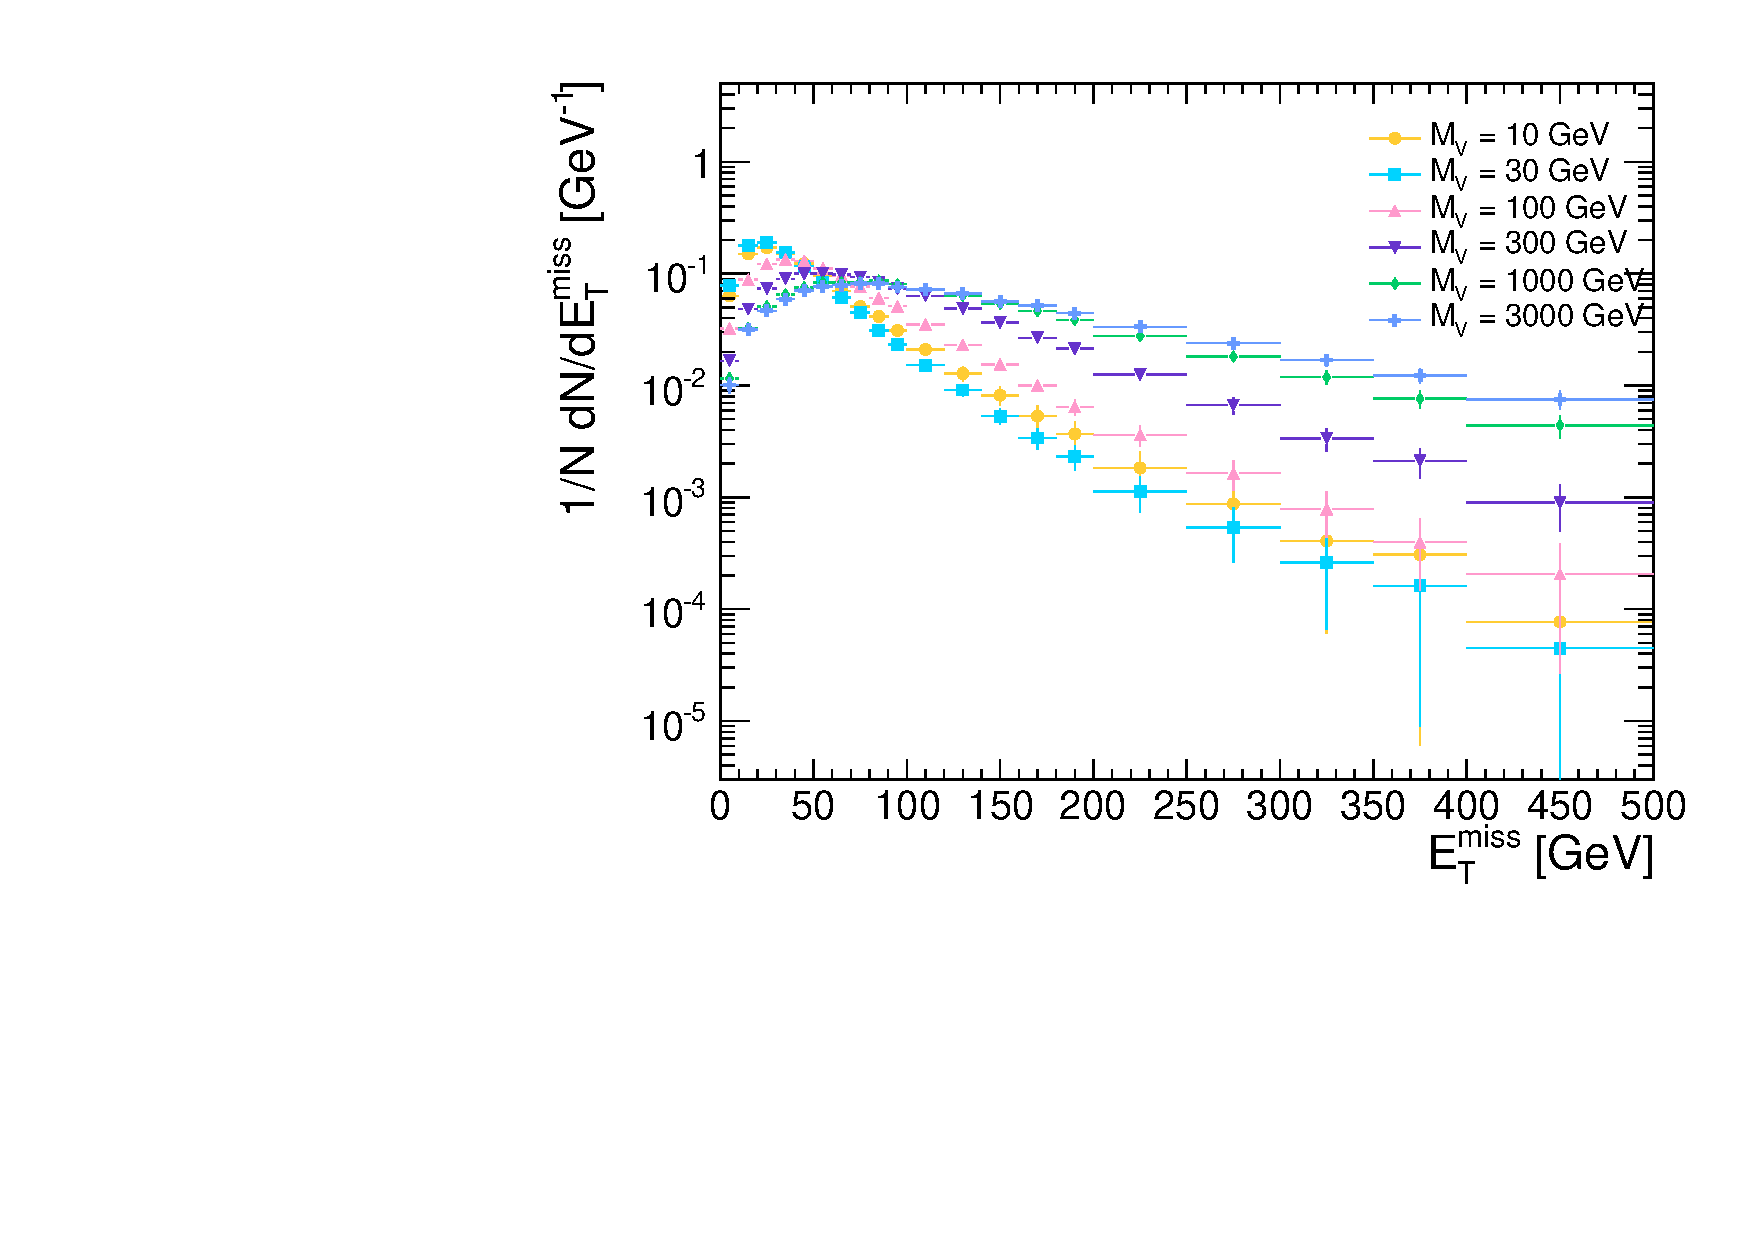
\includegraphics[width=0.49\textwidth]{figures/EW/pt_vv_Mx15}
}    
\hfill
\subfloat[Missing transverse momentum distribution for the hadronic W+\MET final state.\label{fig:DMV_EW_Whad_MET_SVMed}]{%
	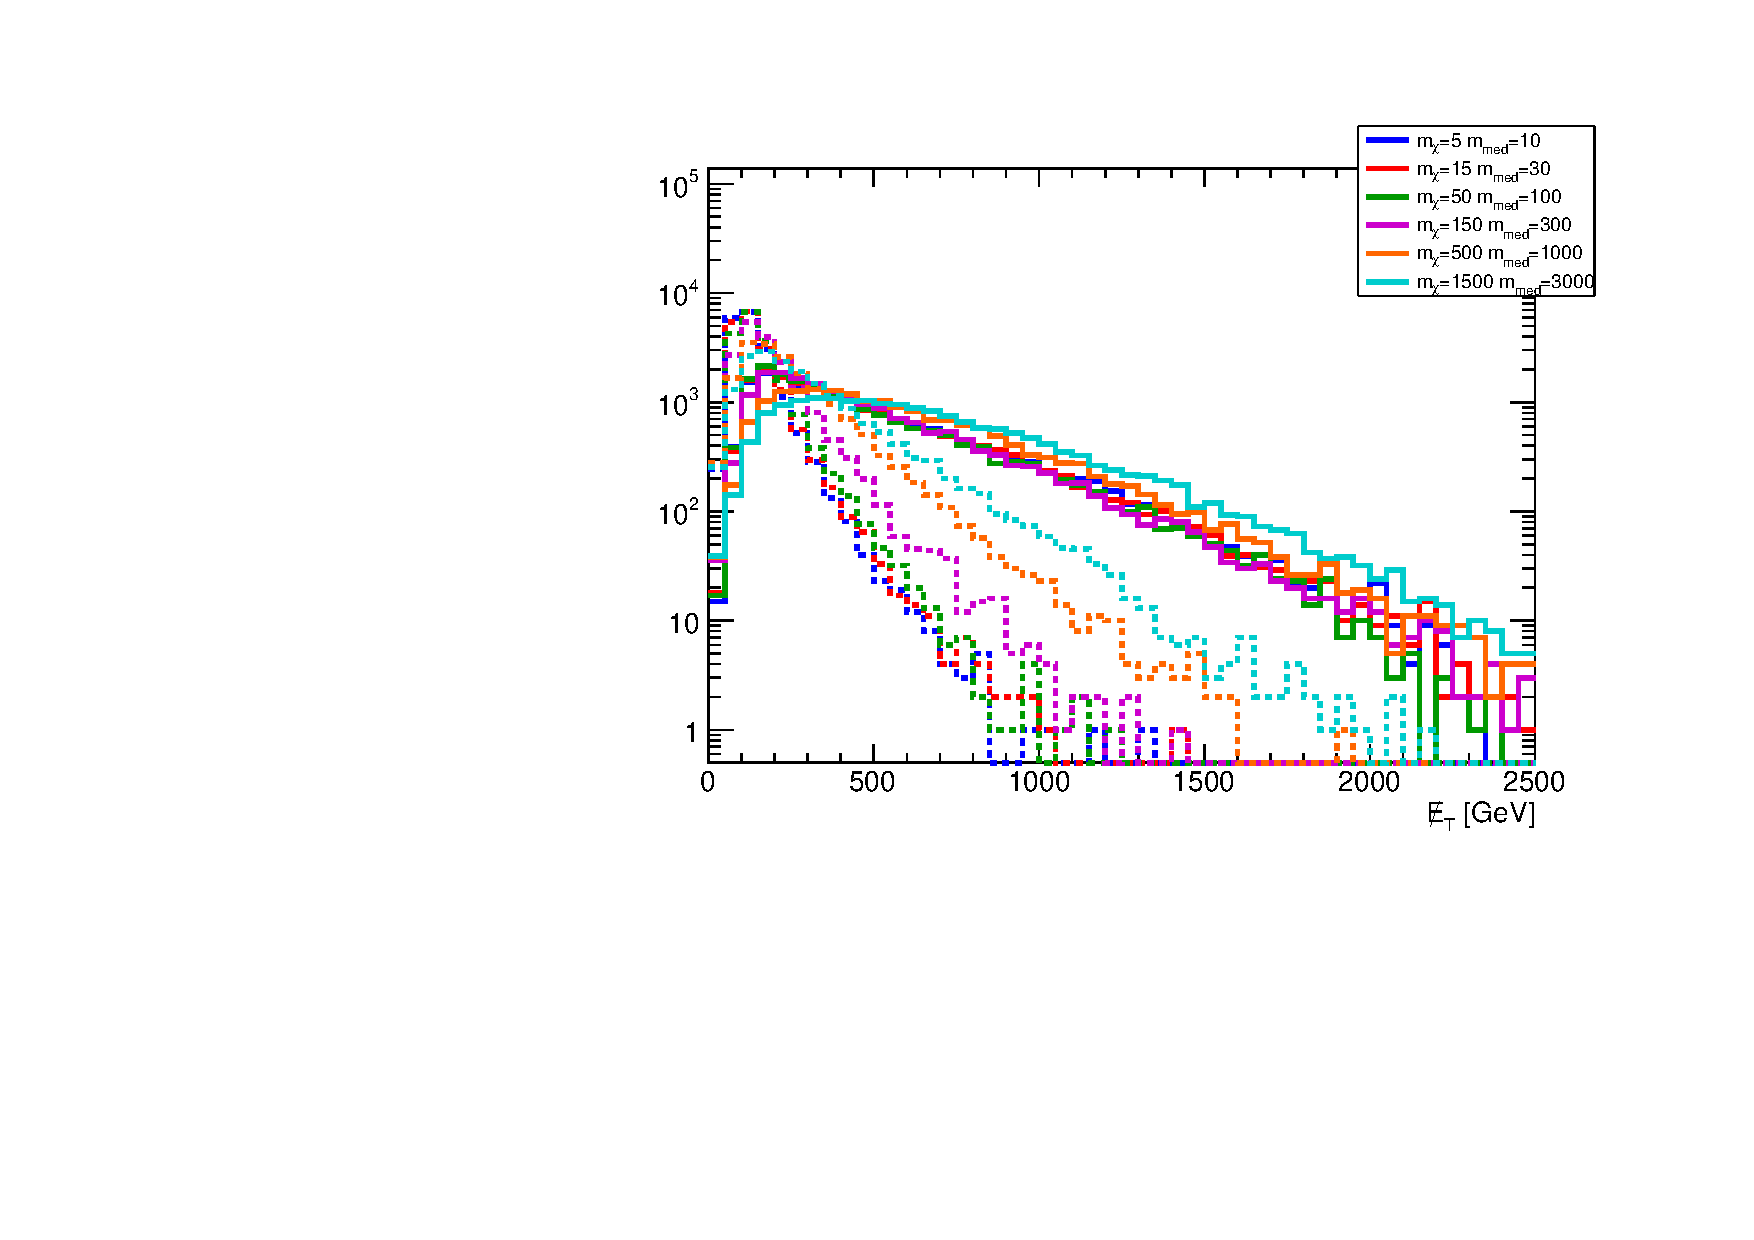
\includegraphics[width=0.49\textwidth]{figures/EW/monoWhad_Destructive/metPt}
}    
\caption{Kinematic distributions relevant for searches with W, Z and photons in the final state, 
for the simplified model
       with a vector mediator exchanged in the \schannel.}
\label{fig:DMV_EW_kinematics_SVMed}
\end{figure*}
